%! TEX root = meet6.tex
% the main TeX file which is intended to compile, :VimtexReload after adjustment
% :h vimtex-tex-root
\documentclass[../main.tex]{subfiles}
% \includeonlyframes{one}
\setbeameroption{hide notes} % Only slides
% \setbeameroption{show only notes} % Only notes
% \setbeameroption{show notes on second screen=right} % Both

\begin{document}
\begin{frame}[c,mybg=placeholder,mytitle=imageplus,mycolor=digiPH_gray,light]
	\frametitle{variabel}
	\boxes{digiPH_gray}{digiPH_writer}{A measurable entity that exhibits more than one level or value}
	\boxes{digiPH_gray}{digiPH_writer}{Relational units of analysis carrying values}

	Konsep yang diterapkan secara empiris dan mempunyai minimal dua macam kemungkinan nilai (value).

	\resizebox{.75\textwidth}{!}{
		\begin{tabular}{cc}
			\hline
			Variabel            &  Nilai  \\
			Jenis kelamin       &  nilai : pria/wanita  \\
			Status perkawinan   &  nilai kawin/belum kwn/janda/duda.  \\
			Bentuk ruang        &  nilai : segi empat, oval  \\

			Luas ruang          &  nilai : ...m2  \\
			Jumlah pengnjung    &  nilai :  .. orang  \\
			Tingkat sinar       &  nilai :  terang/ redup/ gelap  \\
			Kepuasan pelanggan  &  nilai : puas/ sedang / tidak puas  \\
		\end{tabular}}
\end{frame}

\begin{frame}[c,mybg=bgcanvasblue,mytitle=imageplus,light]
	\frametitle{Klasifikasi variabel}
	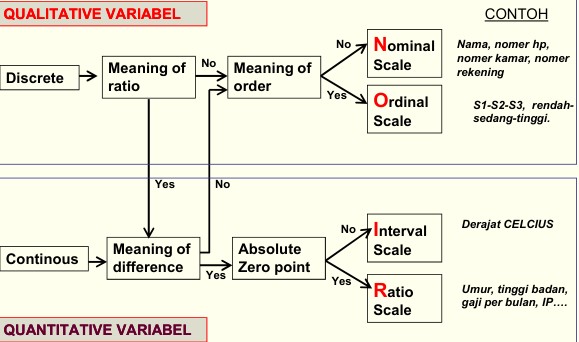
\includegraphics[width=.9\textwidth]{6var}
\end{frame}

\begin{frame}[t,mybg=bg,mytitle=standard,light]
	\frametitle{validitas dan reabilitas}

	\only<1>{\textbf{Validitas:} menunjukkan sejauh mana suatu alat pengukur mengukur apa yang ingin
		diukur.

		- Bila ingin mengukur berat suatu benda, maka harus menggunakan timbangan. Bila ingin
		mengukur tinggi suatu benda, maka harus menggunakan meteran.

		- HAL INI TERLIHAT PADA KUISIONER YANG DIBANGUN -> VALIDITAS DATANYA -> VALIDITAS PENELITIANNYA.}

	\only<2->{\textbf{Reliabilitas:} Indeks yang menunjukkan sejauhmana suatu alat pengukur dapat dipercaya atau dapat diandalkan. Untuk menunjukkan sejauh mana suatu hasil pengukuran tetap konsisten apabila pengukuran diulangi dua kali atau lebih.

			{\small		-  Misal: mengukur lebar rumah dengan 2 jenis alat ukur (a. meteran logam, b. jumlah langkah kaki). Meteran logam akan menunjukkan hasil yang sama ketika mengukur lebar rumah untuk kedua kali atau lebih, sementara jumlah langkah kaki belum tentu sama. Meteran logam -> alat pengukur yang reliabel, sedangkan langkah kaki -> alat pengukur yang tidak reliabel.}}


	\only<3->{\textcolor{blue}{ HAL DI ATAS ADALAH RELIABILITAS DARI ASPEK FISIK, LALU BAGAIMANAKAH IMPLIKASINYA PADA PENELITIAN-PENELITIAN SOSIAL.}}

\end{frame}

\begin{frame}[t,mybg=fgd,light]

	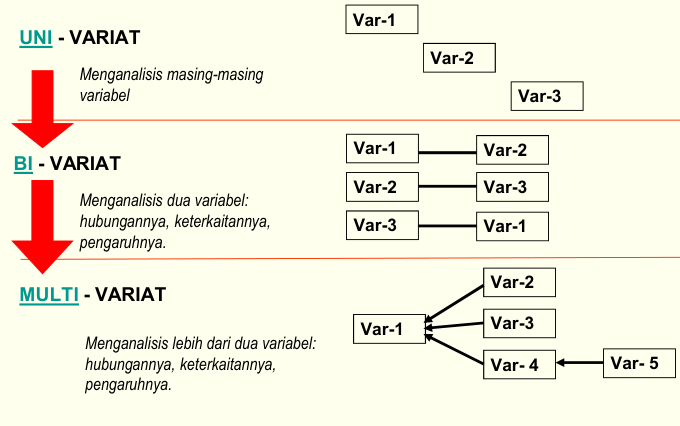
\includegraphics[width=.9\textwidth]{6var2}
\end{frame}

\begin{frame}[t,mybg=fgd,mytitle=center,light]

	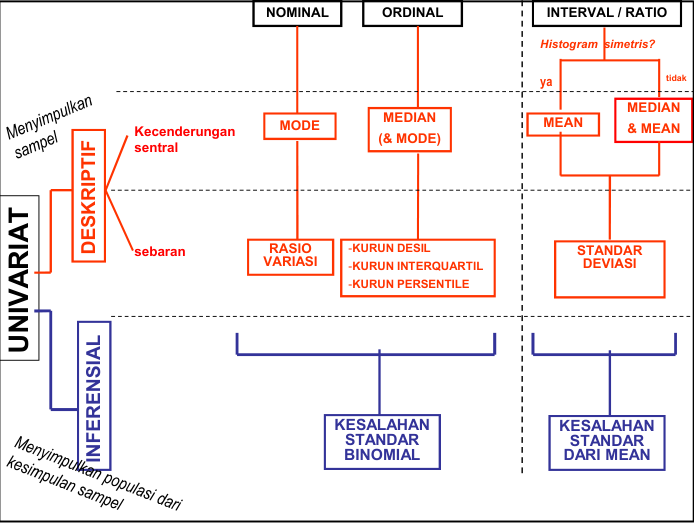
\includegraphics[width=.9\textwidth]{6uni}
\end{frame}

\begin{frame}[t,mybg=fgd,mytitle=center,light]

	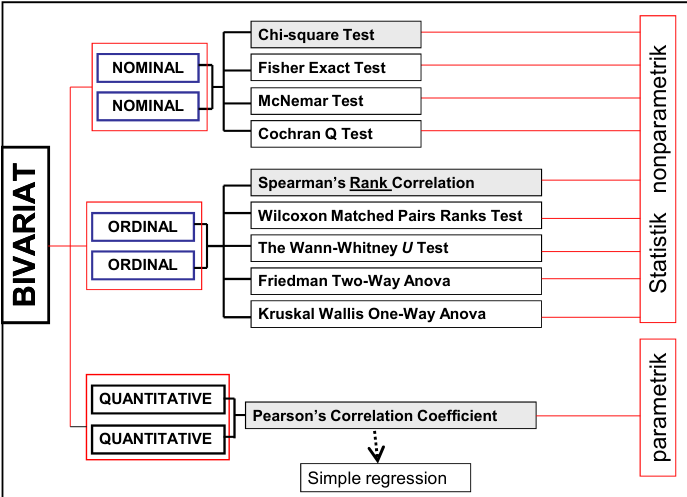
\includegraphics[width=.9\textwidth]{6bi}
\end{frame}

\begin{frame}[t,mybg=fgd,mytitle=center,light]

	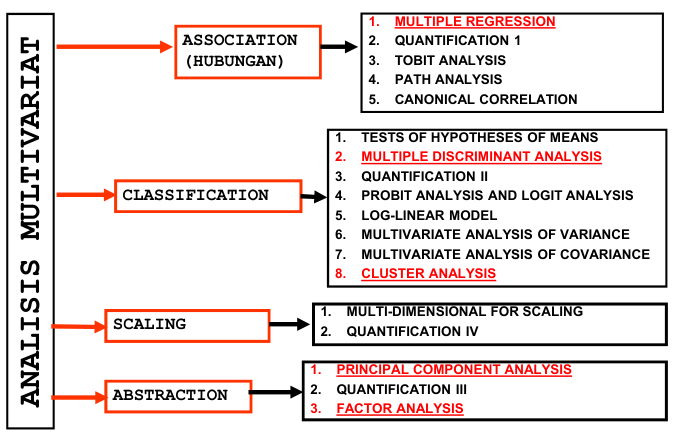
\includegraphics[width=.9\textwidth]{6multi}
\end{frame}

\begin{frame}[label=one,c,mybg=bg3,mytitle=standard,light]%rmve mycolor when use mybg
	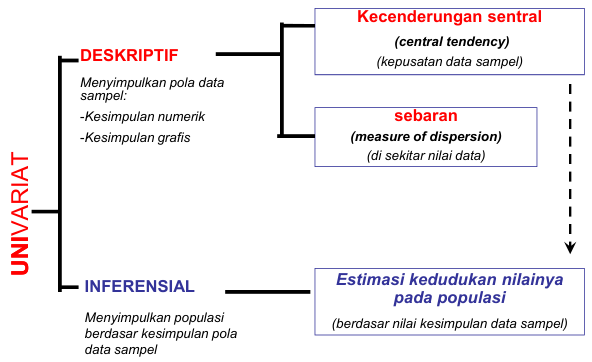
\includegraphics[width=.9\textwidth]{6des}

\end{frame}

\begin{frame}[label=one,t,mytitle=standard,mycolor=digiPH_ocean,dark]%rmve mycolor when use mybg
	\frametitle{Univariat deskriptif}
	\framesubtitle{Variabel nominal}
	Misal : Jumlah kebun menurut jenis tanaman
	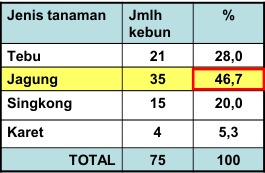
\includegraphics[width=35mm]{6mode}

	\only<1>{\boldwhite{A. Kecenderungan sentral}\\
		hanya mode
		\textbf{Mode}: Kategori berjumlah \textcolor{white}{ terbanyak} atau sering muncul\\
		\textbf{Jadi mode-nya adalah jagung}}

	\onslide<2->{

		\boldwhite{B. Sebaran: rasio variasi (v)}\\
		v = 1.00 - 46,7\%
		\textcolor{red}{ = 0.533}\\
		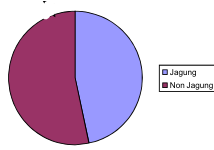
\includegraphics[draft,width=25mm]{6mode2}}

\end{frame}

\begin{frame}[label=one,t,mybg=bg3,mytitle=standard,light]%rmve mycolor when use mybg
	\includegraphics<1>[width=.89\textwidth]{6des2}
	\only<2->{\boldblue{A. Kecenderungan sentral}\\
		median (dan) mode}

	\includegraphics<2->[width=.87\textwidth]{6ord}
\end{frame}

\begin{frame}[label=one,mybg=bg3,mytitle=standard,light]%rmve mycolor when use mybg
	\frametitle{univariat deskriptif: var. ordinal}
	\boldblue{B. Sebaran : desil}
	\begin{columns}
		\begin{column}{0.5\textwidth}
			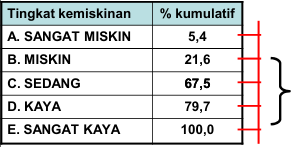
\includegraphics[,width=.9\textwidth]{6ord2}
		\end{column}
		\begin{column}{0.5\textwidth}
			Sebaran desil (decil range) = meliputi kurun kategori-kategori dari posisi 10\% hingga 90\% (kumulatif)\\
			\textcolor{blue}{Posisi 10\% terletak di B (nilai antara  5,4\% - 21,6\%)}\\

			\textcolor{blue}{  Posisi 90\% terletak di E (E bernilai antara 79,7\% -
				100\%)}

			\textbf{Jadi sebaran desil dari B(miskin) sampai dengan E (sangat kaya).}

		\end{column}
	\end{columns}

\end{frame}

\begin{frame}[label=one,mybg=bg3,mytitle=standard,light]%rmve mycolor when use mybg

	\frametitle{univariat deskriptif: var. ordinal}
	\begin{columns}
		\begin{column}{0.5\textwidth}
			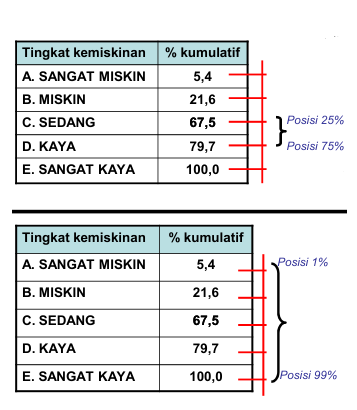
\includegraphics[,width=.9\textwidth]{6ord3}
		\end{column}
		\begin{column}{0.5\textwidth}
			\boldblue{B. Sebaran : interquartile}
			Sebaran interquartile (interquartile range) = meliputi kurun kategori-kategori dari posisi 25\% hingga 75\% (kumulatif)\\

			\textbf{Jadi sebaran interquartile dari C (sedang) sampai dengan D (kaya)}\\
			\boldblue{B. Sebaran : persentil}
			Sebaran persentil (persentil range) = meliputi kurun kategori-kategori dari posisi 1\% hingga 99\% (kumulatif) atau di potong 1\% bawah dan 1\% atas.\\

			\textbf{Jadi sebaran persentil sangat miskin sampai dengan sangat kaya.}

		\end{column}
	\end{columns}

\end{frame}





\end{document}
